%\modeCorrection


\renewcommand{\thesubsection}{\textcolor{red}{\Roman{section}.\arabic{subsection}}}
\renewcommand{\thesubsubsection}{\textcolor{red}{\Roman{section}.\arabic{subsection}.\alph{subsubsection}}}
\renewcommand{\titreDocu}[1]{
  \refstepcounter{document} % update counter
  \textbf{Exercice \arabic{document} -- #1} 
  \addcontentsline{toc}{document}{\protect\numberline{} #1} % update table of content
}

\setcounter{section}{0}
\setcounter{document}{0}


\nomPrenomClasse
\vspace{1cm}

\begin{center}
\begin{mdframed}[style=titr, leftmargin=60pt, rightmargin=60pt, innertopmargin=7pt, innerbottommargin=7pt, innerrightmargin=8pt, innerleftmargin=8pt]
\begin{center}
\begin{Large}
    Devoir Surveillé : Corps purs et mélanges au quotidien (55min)
\end{Large}
\end{center}
\end{mdframed}
\end{center}
\vspace{1cm}

\begin{tableauCompetences}
    APP & S'approprier les informations d'un document & & & & \\
    \hline
    REA & Utiliser les pourcentages et les fractions  & & & & \\
     \hline 
    ANA &  Exploiter les informations extraites des données & & & & \\
    \hline
    VAL & Valider/critiquer un modèle & & & &
\end{tableauCompetences}

\begin{tcolorbox}[colback=red!5!white,colframe=red!75!black,title=\textbf{Consignes : }]
   \begin{enumerate}
       \item Vous rendrez l'énoncé avec votre copie de rédaction.
       \item Lisez-bien l'énoncé des exercices. Les questions sont pour la plupart indépendantes. Si vous bloquez sur une question, passez à la suivante,
       \item N'oubliez pas les unités dans vos résultats.
   \end{enumerate}
\end{tcolorbox}

\begin{doc}{Le cyclohexane \begin{large}
    /9,5 points
\end{large}}
Le cyclohexane est une espèce chimique incolore très utilisée en chimie organique pour la synthèse d'arôme artificiel par exemple.
\begin{center}
    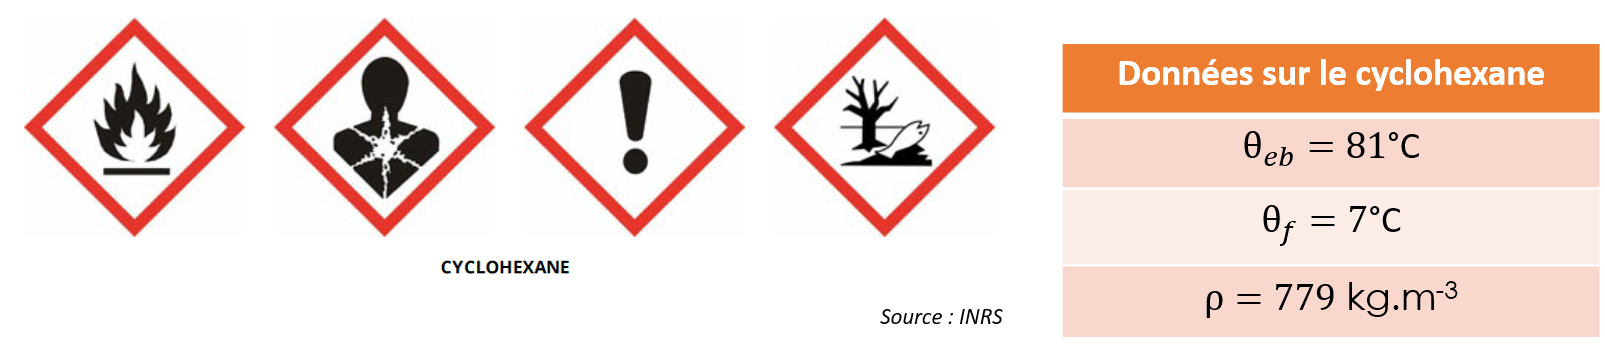
\includegraphics[scale=0.5]{Images/Cyclohexane.png}
\end{center}

\question{Représenter deux pictogrammes de sécurité sur votre copie et donner leur signification. (2pts)}{De gauche à droite sur la figure : inflammable, toxicité aigu (agent CMR), irritant/nocif, pollue l'environnement.}{0}
%\\
\question{Le cyclohexane est très volatil (il s'évapore à l'air libre). Quels sont les Equipements de Protection Individuels (EPI) à utiliser pour manipuler ce produit ? (1pt)}{Blouse, gants, lunettes et hotte protectrice (car volatil).}{0}
%\\
\question{Donner la signification \underline{précise} du symbole \og $\theta_{f}$ \fg. (1pt)}{Il s'agit de la température de fusion, c'est-à-dire la température à partir de laquelle le cyclohexane devient liquide.}{0}
%\\
\question{Avec quel instrument peut-on mesurer $\theta_{f}$ ? (1pt)}{Avec un banc Kofler (attention à l'écriture).}{0}
%\\
\question{Justifier que le cyclohexane est liquide à la température $T=20\degreCelsius$. (1pt)}{D'après les données fournies, la température de 20$\degreCelsius$ est supérieure à la température de fusion $\theta_{f}$ et inférieure à la température d'ébullition $\theta_{eb}$. Le cyclohexane est donc bien liquide.}{0}
%\\
\question{Citer la masse volumique de l'eau en kg.m$^{-3}$.(0,5pt)}{La masse volumique de l'eau est $\rho_{eau}=1000$~kg.m$^{-3}$.}{0}
%\\
\question{En déduire la densité $d$ du cyclohexane. (1pt)}{La densité du cyclohexane est donc :
\begin{equation*}
    d = \frac{779}{1000}=0,779
\end{equation*}}{0}
%\\
\question{Sachant que le cyclohexane \underline{n'est pas miscible} avec l'eau, schématiser une éprouvette graduée avec un mélange eau-cyclohexane (2pts).}{\begin{center}
    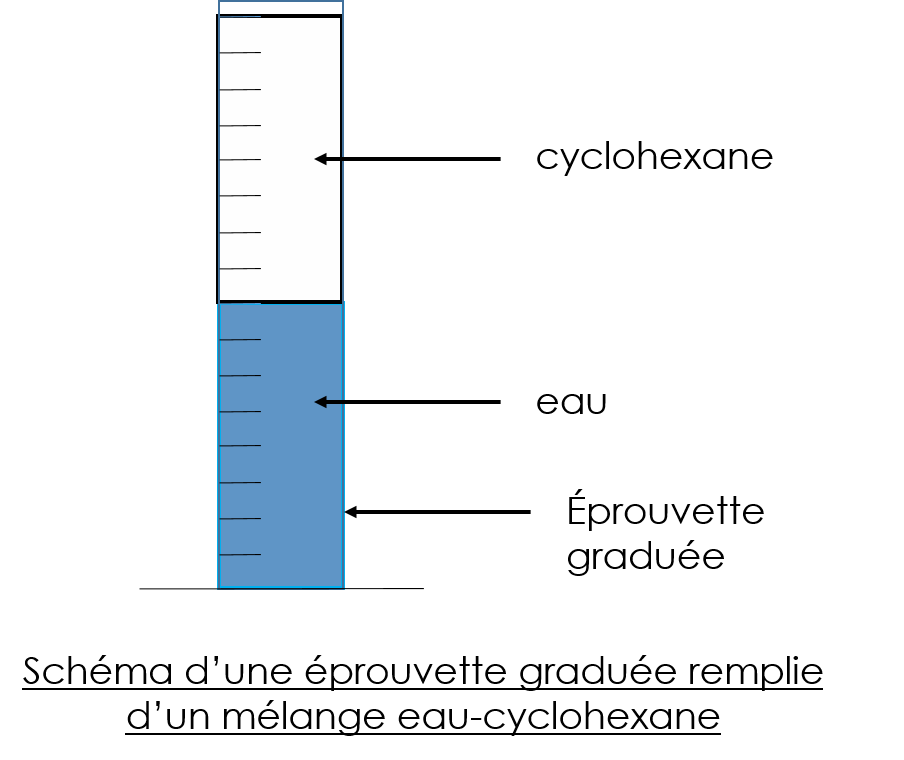
\includegraphics[scale=0.5]{Images/Eprouvette_solution.png}
\end{center}}{0}
\end{doc}

\begin{doc}{L'huile essentielle d'orange\begin{Large}
    /4,5 points
\end{Large}}
\begin{wrapfigure}{r}{0.3\textwidth}
\vspace{-1cm}
    \centering
      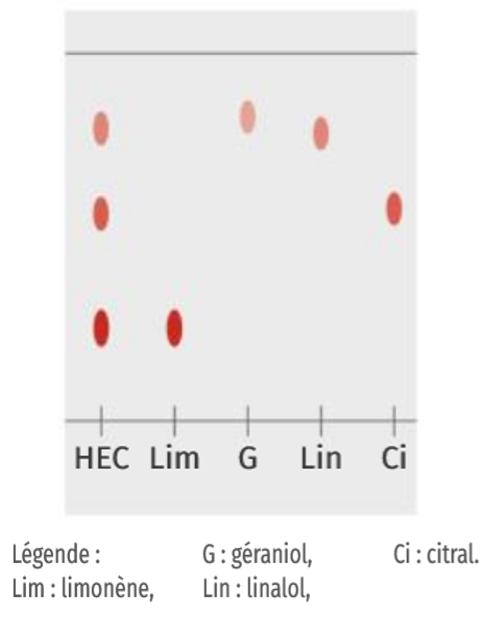
\includegraphics[scale=0.65]{Images/CCm_HEO_3.png}
  \end{wrapfigure}
L'huile essentielle de citron (notée HEC) est obtenue par un procédé mécanique appelé \og extraction par expression à froid\fg~. Cette technique est réservée spécifiquement aux agrumes en raison de la localisation de leurs huiles essentielles (principalement dans la peau).\\
On réalise une CCM afin d'identifier les espèces chimiques présentes dans ces huiles essentielles. Le résultat de la CCM est observable sur la figure de gauche.\\

\question{Rappeler la signification du sigle \og CCM \fg. (0,5pt)}{CCM = Chromatographie sur Couche Mince}{0}
%\\
\question{Que permet de faire la CCM ? (1pt)}{La chromatograpie sur couche mince permet de \textbf{séparer} et d'\textbf{identifier} des espèces chimiques au sein d'un mélange homogène.}{0}
%\\
\question{En vous appuyant sur le résultat de la CCM, justifier que l'huile essentielle de citron (HEC) est un mélange. (1pt)}{On voit apparaître 3 tâches lors de la migration des espèces avec l'éluant correspondant à trois espèces chimiques différentes contenues dans HEC. HEC est donc composé de plusieurs espèces chimiques ce qui est la définition d'un mélange.}{0}
%\\
\question{En vous appuyant sur la légende de la figure, déterminer les espèces chimiques présentes dans l'huile essentielle de citron. (2pts)}{En regardant les espèces avec un même rapport frontal que ceux présents dans HEC, on en déduit qu'il y a du limonène, du linalol et du citral dans HEC.}{0}
\end{doc}

\begin{doc}{Les solutions antisceptiques \begin{Large}
    /6 points
\end{Large}}
Les solutions d’eau oxygénée sont des mélanges d’eau et de peroxyde d’hydrogène \chemform{H_2O_2}. Les solutions d’eau oxygénée à usage domestique, utilisées pour nettoyer et désinfecter les plaies, ont généralement un pourcentage en masse de peroxyde d’hydrogène égal à 3\%. Cependant, les solutions d’eau oxygénée à usage industriel sont plus concentrées : leur pourcentage en masse de peroxyde d’hydrogène peut atteindre 30\%, et même plus.\\

La courbe ci-dessous représente l’évolution de la masse volumique d’une solution d’eau oxygénée en fonction de sa proportion (ou pourcentage) en masse de peroxyde d’hydrogène :

\begin{center}
    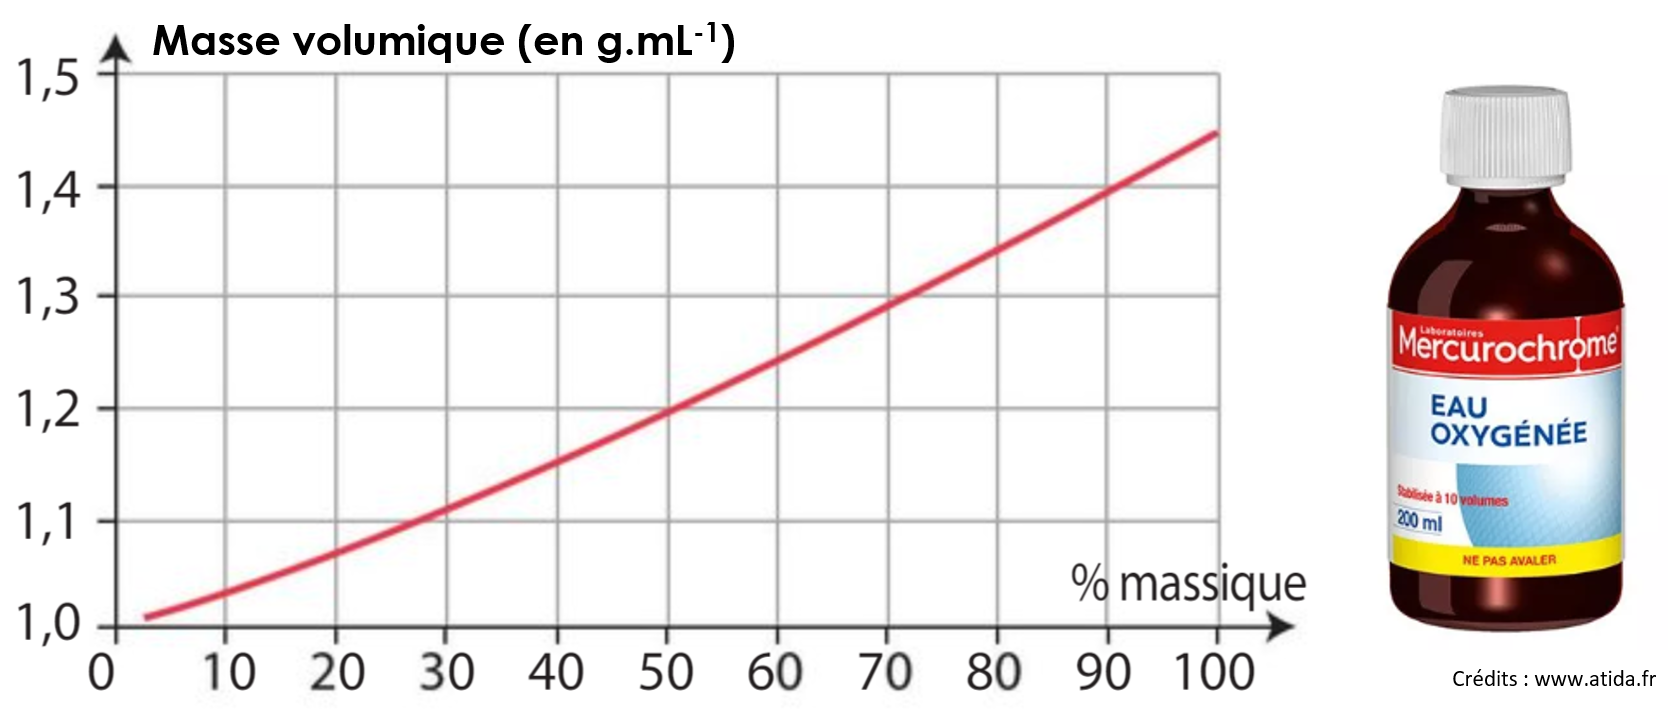
\includegraphics[scale=0.4]{Images/Peroxyde_hydrogene.png}
\end{center}

Afin de déterminer le pourcentage en masse de peroxyde d’hydrogène d’une solution d’eau oxygénée à usage industriel, on détermine la masse d’un volume $V_{H_2O_2} = 25$~mL de cette solution : $m_{H_2O_2} = 30$~g.\\
\question{Nommer le matériel qu'il faut utiliser pour réaliser les mesures précédentes. (2pts)}{Pour mesurer la masse : une balance. Pour mesurer un volume, une éprouvette graduée ou une fiole jaugée (qui est plus précise).}{0}
%\\
\question{Calculer la masse volumique $\rho_{indus}$ de la solution d’eau oxygénée à usage industriel étudiée. (1pt)}{On sait d'après le cours que $\rho=\frac{m}{V}$ soit avec les notations de l'énoncé : $\rho_{indus}=\frac{m_{H_2O_2}}{V_{H_2O_2}}=\frac{30}{25}=1,2$~g.mL$^{-1}$.}{0}
%\\
\question{Déterminer graphiquement la proportion (ou pourcentage) en masse de peroxyde d’hydrogène de la solution d’eau oxygénée à usage industriel étudiée. (1,5pt)}{A l'aide du graphique, on lit un pourcentage en masse pour une masse volumique de $1,2$~g.mL$^{-1}$ égale à 50\%.}{0}
%\\
\question{Calculer le volume de solution d’eau oxygénée à usage industriel contenant $m_2=16$~g de peroxyde d’hydrogène. (1,5pts)}{On sait que la masse volumique correspondante est $\rho_{indus}=1,2$~g.mL$^{-1}$. On en déduit $V=\frac{m_2}{\rho_{indus}}=\frac{16}{1,2}=13$~mL.}{0}
\end{doc}
\newpage
\begin{doc}{La face cachée de l'iceberg  \begin{Large}
    /5 points
\end{Large}}
\begin{wrapfigure}{r}{0.3\textwidth}
\vspace{-1cm}
    \centering
      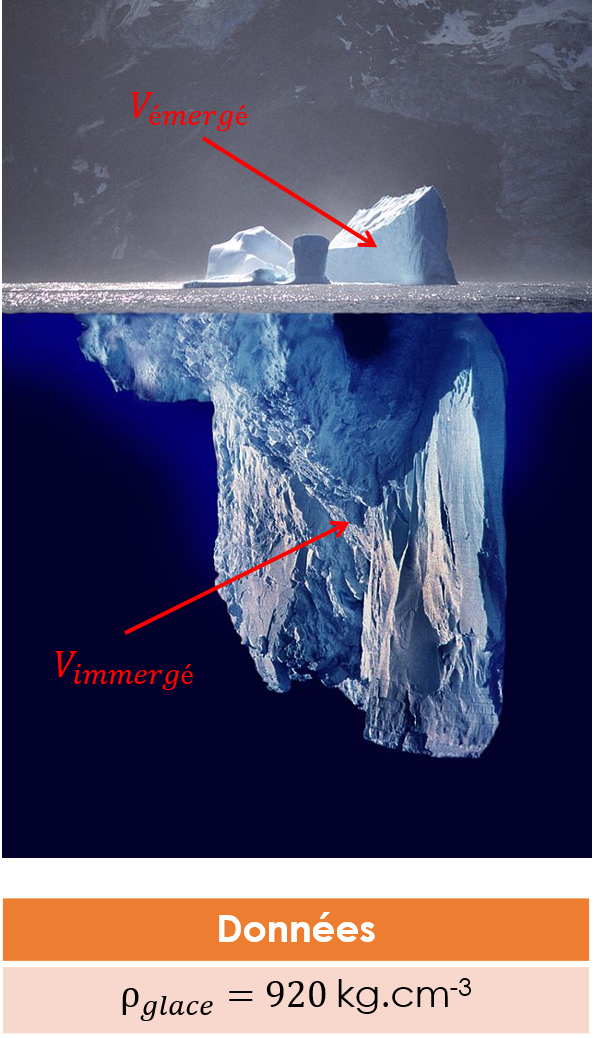
\includegraphics[scale=0.5]{Images/Iceberg.png}
  \end{wrapfigure}
On appelle \og volume immergé \fg, noté $V_{\text{immergé}}$, d'un iceberg le volume de cet iceberg se situant sous l'eau. De même, on appelle \og volume émergé \fg~ d'un iceberg la partie de cette iceberg flottante sur l'eau. Un petit modèle mécanique permet d'établir :
\begin{equation*}
    \rho_{glace}\times V_{Tot} = \rho_{eau}\times V_{\text{immergé}}
\end{equation*}
avec $V_{Tot}$ le volume total de l'iceberg.\\
\question{Donner la relation entre le volume total $V_{Tot}$ de l'iceberg, $V_{\text{immergé}}$ et $V_{\text{émergé}}$. (1pt)}{$V_{Tot}=V_{\text{immergé}}+V_{\text{émergé}}$}{0}%\\
\question{Déterminer l'expression littérale de la proportion du volume immergé de l'iceberg, noté $x_V(\text{immergé})$, en fonction de $\rho_{glace}$ et $\rho_{eau}$. \`{A} l'aide des données, calculer cette proportion. (3pts)}{La proportion volumique du volume immergé est donné par la formule : 
\begin{equation*}
    x_V(\text{immergé}) = \frac{V_{\text{immergé}}}{V_{Tot}}
\end{equation*}
Soit avec l'équation donnée par l'énoncé :
\begin{equation*}
    x_V(\text{immergé}) = \frac{\rho_{glace}}{\rho_{eau}} = \frac{920}{1000} = 92\%
\end{equation*}}{0}%\\
\question{Valider votre résultat en regardant la figure. (1pts)}{Le résultat obtenu est cohérent avec la partie du volume immergé qu'on peut voir sur la figure.}{0}
\end{doc}
